% PLL block diagram: Phase Detector → Loop Filter → output, VCO feedback
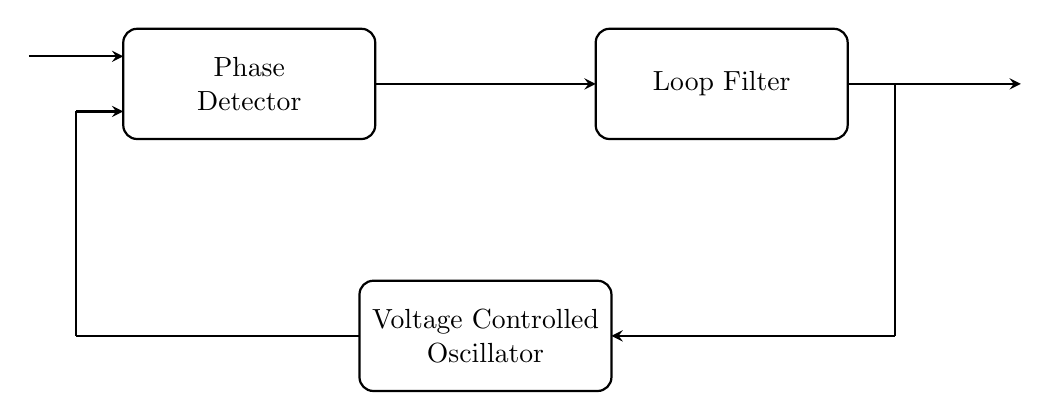
\begin{tikzpicture}[
	box/.style={
		draw, rounded corners=5pt, thick,
		minimum width=3.2cm, minimum height=1.4cm,
		align=center, font=\normalsize
	},
	arr/.style={->, >=stealth, thick},
	line/.style={thick}
]

% Nodes
% PD centre (0,0):  west=(-1.6,0), east=(1.6,0)
% LF centre (6,0):  west=(4.4,0),  east=(7.6,0)
% VCO centre (3,-3.2): west=(1.4,-3.2), east=(4.6,-3.2)
\node[box] (pd)  at (0,   0)    {Phase\\Detector};
\node[box] (lf)  at (6,   0)    {Loop Filter};
\node[box] (vco) at (3,  -3.2)  {Voltage Controlled\\Oscillator};

% Input signal — horizontal arrow into PD, slightly above centre
\draw[arr] (-2.8,  0.35) -- (-1.6,  0.35);

% PD → LF
\draw[arr] (1.6, 0) -- (4.4, 0);

% LF east → junction (0.6 cm outside box) → output arrow
\draw[line] (7.6, 0) -- (8.2, 0);
\draw[arr]  (8.2, 0) -- (9.8, 0);

% Right vertical: junction down to VCO row
\draw[line] (8.2,  0)   -- (8.2, -3.2);

% Arrow from right side into VCO east
\draw[arr]  (8.2, -3.2) -- (4.6, -3.2);

% VCO west → left to left-side vertical
\draw[line] (1.4, -3.2) -- (-2.2, -3.2);

% Left vertical up, then short horizontal arrow into PD, slightly below centre
\draw[line] (-2.2, -3.2) -- (-2.2, -0.35);
\draw[arr]  (-2.2, -0.35) -- (-1.6, -0.35);

\end{tikzpicture}
